\documentclass[9pt,a4paper]{article}
\usepackage[utf8]{inputenc}       
\usepackage[english,russian]{babel}
%\usepackage{PTSerif}                
\usepackage[pdftex]{graphicx}        
\usepackage{layout}                   
\usepackage{fancyhdr}                  
\usepackage{fullpage}                   
\usepackage{array}                       
\usepackage{longtable}                    
\usepackage{verbatim}                      
\usepackage{footnote}                       
                                             
\setlength\voffset{-1in}                      
\setlength\hoffset{-1in}                       
\setlength\topmargin{1cm}                       
\setlength\oddsidemargin{2cm}                    
\setlength\textheight{25.7cm}                     
\setlength\textwidth{17.001cm}                     
\setlength{\topskip}{1.3cm}                         
\setlength\headheight{0cm}                           
\setlength\headsep{0cm}                               
                                                       
\pagestyle{fancyplain}                                  
\fancyhf{}                                               
\cfoot{\small\em \textcopyright \hspace{0.1em} ARCСN 2013}
\rfoot{\small \thepage}

\renewcommand{\labelitemii}{$\circ$}
                                      
\title{Описание HCProbe}
\author{Александр Вершилов}

\begin{document}
\maketitle
\begin{figure}[!h]
   \centering 
   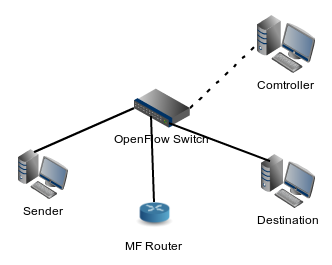
\includegraphics[width=0.3\columnwidth]{images/testcfg2.png}
\end{figure}                                                        

\tableofcontents

\pagebreak
\section{Общее описание}
HCProbe программа для реализиции софтового OpenFlow свича и простой
генерации разбору OpenFlow сообщений.

\section{EDSL}

\appendix{Примеры программ}
\end{document}
